\documentclass{acaces}

\usepackage{tikz}
\usetikzlibrary{shapes.multipart}

\begin{document}


\title{Data Aware Embedded \\Machine Learning
}

\author{
    Emil~Njor\addressnum{1}\comma\extranum{1},
    Jan~Madsen\addressnum{1}\comma\extranum{2},
    Xenofon~Fafoutis\addressnum{1}\comma\extranum{2}
}

\address{1}{
    Danmarks Tekniske Universitet,
    Richard Petersens Plads,
    Building 322,
    2800 Kongens Lyngby,
    Denmark
}

\extra{1}{E-mail: emjn@dtu.dk, Phone: +4560699096}
\extra{2}{Supervisor}

\pagestyle{empty}


\begin{abstract}
    In this poster abstract I introduce my research into Data Aware Embedded Machine Learning.
    The idea of Data Aware Embedded Machine Learning is to make embedded machine learning systems that take into account the resource consumption of its input data.
    This can be used to improve the predictive performance of a machine learning system under some given resource constraints, or to reduce the overall resource consumption of an embedded machine learning system.
    Under this research field I present my work and ideas of Data Aware Neural Architecture Search, Data Aware Datasets, and Data Aware Neural Networks.
\end{abstract}
\newline
\keywords{Embedded Machine Learning, Data Aware Methods, Data Aware NAS, Data Aware Datasets, Data Aware Neural Network}

\section{Introduction}
Embedded Machine Learning, also known as tinyML, is a research field aiming to bring complex machine learning models to embedded devices. 
The research field is still in its infancy, but has already shown promising results in a wide range of applications, such as keyword spotting, image classification, and predictive maintenance.

The main challenge of embedded machine learning is to make machine learning work well in the constrained resources, such as memory, compute, and energy, of embedded devices.
Most research in the field has tried to solve this challenge by reducing the resource consumption of the machine learning models themselves - especially the resource hungry models such as neural networks and their variants.
This has e.g., been achieved using methods such as quantization, pruning and neural architecture search\cite{njor2022primer}.

However, the resource consumption of the machine learning model is only a part of the resource consumption of the entire machine learning system.
A typical embedded machine learning tasks consists of collecting data from a sensor, pre-processing this data, running the machine learning model, and taking some action based on the output of the machine learning model.

In my research I work with the data granularity of the input data captured, pre-processed and given to the machine learning model.
At the core of this research is the idea that input data can be configured to be more or less resource intensive.

E.g., sound data can be captured at different sample rates.
Likewise, image data can be captured at different resolutions.
Higher sample rates and image resolutions will be more resource intensive, but will also contain more information that may be valuable to the machine learning model.
On the other hand, lower sample rates and image resolutions will be less resource intensive, but will also contain less information.

This idea can be used to reduce the resource consumption of an embedded machine learning system, but also to improve the performance of a machine learning system under some given resource constraints.
I have thought the name "Data Aware Embedded Machine Learning" suitable to describe this research direction.

In the following sections of this poster abstract I will describe my work and ideas for work in this research direction in more detail.
In particular, I will introduce:
\begin{description}
    \item[Data Aware Neural Architecture Search] An extension of Neural Architecture Search that simultaneously searches for an optimal combination of a Neural Network Architecture and a Data Granularity.
    \item[Data Aware Datasets] Datasets that support easy loading of multiple data granularities.
    \item[Data Aware Neural Networks] Specialized Neural Networks that can run inference of multiple data granularities.
\end{description}

\section{Data Aware Neural Architecture Search}
The idea of a Data Aware Neural Architecture Search builds on top of Neural Architecture Search.
Simply put, a Neural Architecture Search is a computer program that searches for an optimal Neural Network Architecture for a given task.

A Data Aware Neural Architecture Search extends this by searching for an optimal combination of a Data Granularity and Neural Network Architecture for a given task.
This extension enables scaling the resource consumption of the Data Granularity up or down to either give more information to the Neural Network Architecture, or to allocate resources to the Neural Network Architecture.
This should enable a Data Aware Neural Architecture Search to find Machine Learning Systems that perform better at a given amount of available resources.
Figure~\ref{fig:dnas} shows a comparison of Data Aware Neural Architecture Search, the concept of AutoML and traditional Neural Architecture Search.

\begin{figure}
    \centering
    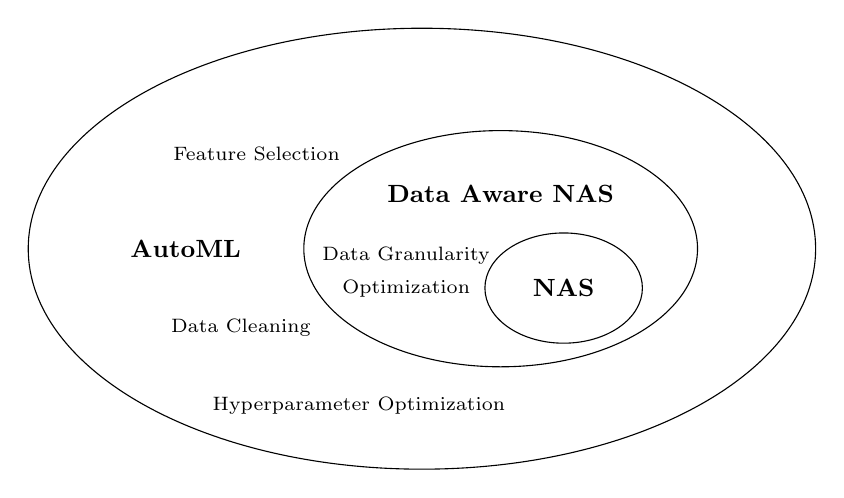
\begin{tikzpicture}[every text node part/.style={align=center}]
        \draw ellipse (5 and 2.8);
        \node at (-3,0) {\small \textbf{AutoML}};
        \node at (-0.8, -2) {\scriptsize Hyperparameter Optimization};
        \node at (-2.1, 1.2) {\scriptsize Feature Selection};
        \node at (-2.3, -1) {\scriptsize Data Cleaning};
        \draw (1, 0) ellipse (2.5 and 1.5);
        \node at (-0.2, -0.3) {\scriptsize Data Granularity\\\scriptsize Optimization};
        \node[] at (1,0.7) {\small \textbf{Data Aware NAS}};
        \draw (1.8, -0.5) ellipse (1 and .7);
        \node[] at (1.8,-0.5) {\small \textbf{NAS}};
    \end{tikzpicture}
    \caption{The relationship between Data Aware Neural Architecture Search, AutoML and Neural Architecture Search.}
    \label{fig:dnas}
\end{figure}

The idea of Data Granularity is not new.
Even so, many publications and works in the field of machine learning does not consider the Data Granularity of the input data, and simply use the full granularity of the data that they have available.
This can often lead to using more resources on data than necessary. 
E.g., a 2016 paper claims that sample rates used in the literature is up to 57\% higher than necessary \cite{khan2016optimising}.
Considering this, it is also likely that a Data Aware Neural Architecture Search can lower resource consumption for such machine learning systems without sacrificing performance.

A disadvantage of a Data Aware Neural Architecture Search is that the search space is larger than a Neural Architecture Search.
Normally this would be a problem, as Neural Architecture Searches are notoriously slow due to the long training times of many models.
However, the Neural Network models used for embedded devices are often much smaller, and faster to train, which mitigates this issue.

I explored the idea of a Data Aware Neural Architecture Search in a 2023 paper of the same name \cite{njor2023data}.

\section{Data Aware Datasets}
Many datasets used in machine learning are only natively available at a single data granularity.
While it is often possible to manually decrease the data granularity of a dataset e.g., by down sampling or cropping, this is rarely performed.
This is likely due to the fact that it is not always trivial to perform this data granularity reduction, or that machine learning engineers simply do not consider the option.
As the ease of use of a technique such as this is important for adoption, it is likely that datasets that natively support multiple data granularities will be important for the adoption of Data Aware Embedded Machine Learning.

I am currently participating in a project about creating a new version of the visual wake words dataset\cite{chowdhery2019visual} where we may choose to support different data granularities.

\section{Data Aware Neural Networks}
The idea of a Data Aware Neural Network is to create a Neural Network that can run inference on multiple data granularities.
This could be useful in a situation where the data granularity of the input data can be changed dynamically.
E.g., in a factory setting where some operations may require higher data granularities to detect errors, while other operations may not require such high data granularities, where the data granularity can be reduced to reduce resource consumption.

The main challenge of creating a Neural Network that can work with different data granularities is that the network must be able to work with different input sizes.
Drawing inspiration from the field of one-shot Neural Architecture Search, it is possible to create a large super network which several subnetworks can be extracted from\cite{pham2018efficient}.
Such a super network could be trained for the highest data granularity and subnetworks could be extracted, and possibly retrained, for lower data granularities.

I have not yet to start a project to explore this idea in greater detail, and it may not be possible to pursue this during the last year of my Ph.D. studies.
I am however, still looking for someone to help me explore this idea.


\bibliography{bibliography}

\end{document}